\documentclass[tikz]{standalone}
\usepackage{pgfplots}
%\pgfplotsset{width=7cm,compat=1.18}
\usepgfplotslibrary{statistics}
\def\axisdefaultwidth{6cm}
\def\axisdefaultheight{6cm}
%\pgfplotsset{every axis/.style={scale only axis}}

\begin{document}
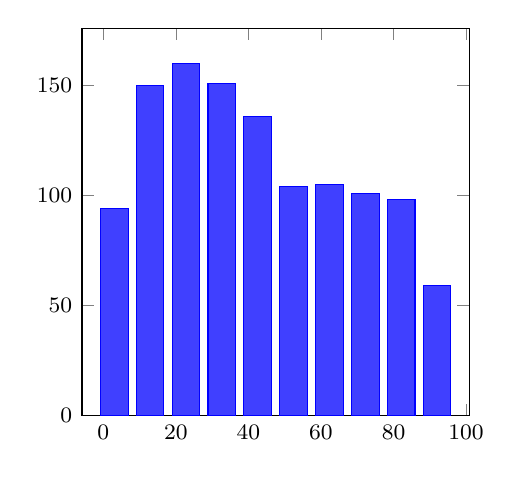
\begin{tikzpicture}
%\begin{axis}[small,ymin=0,title=\texttt{ft}]
\begin{axis}[small,ymin=0]
\addplot [
ybar,
fill=blue!75,
draw=blue]
table [x=perf, y=cnt] {
cnt                 perf                
94.00000            3.00000             
150.00000           12.88600            
160.00000           22.77200            
151.00000           32.65800            
136.00000           42.54400            
104.00000           52.43000            
105.00000           62.31600            
101.00000           72.20200            
98.00000            82.08800            
59.00000            91.97400            
};
\end{axis}
\end{tikzpicture}
\end{document}
